\chapter{Background on Question Answer Systems}

\paragraph{}
Even with the simplifications developed for searching information online it can be tough and time consuming to navigate through the vast amount of data. One of the solutions, to this problem is developing an automated system which is capable enough to accept input in natural language and generate an output which is equally natural. This is where a Question Answer System plays an important role. The aim of a Question Answer System is basically to allow a user to ask a question in everyday language and receive an answer in user comprehensible format. 

\paragraph{}
As with developing software systems, building a efficient and robust Question Answering System has its own fair share of challenges. There are multiple ways in which we can build this system from  machine language translation \cite {bao2014knowledge}, neural networks \cite{iyyer2014neural} and different machine learning algorithms \cite{zhang2003question}.

The first challenge faced while developing such a system is how do we collect the data, how do we store it. The next challenge which comes to mind are the users of this system. A system used developed for the internet needs to effective enough to process the data in a way so as to not restrict the users, in other words the system needs to handle the different ways which users can express themselves. The comes the most challenging aspect of this system, the language itself. We have about 7000 languages spoken world wide, getting data of sufficient quality so that we develop such a system is a difficult task as except a few, most of the languages have minimal resources on the world wide web.
 
\paragraph{}
Below we explain in brief the architecture of a Question Answer System and discuss the different approaches which are used to extract information while implementing a Question Answer System. In general, any such system will always have the following modules,

\begin{enumerate}
\item The Information Retrieval module is responsible for extracting data from different sources, a collection of documents, text, transcripts or a relational database
\item Data Processing module, the system needs to retrieve the data and extract information from it, this involves multiple phases from extracting text data like summaries the performing part of speech tagging, using some chunking to recognize named entities like persons, organizations or locations, and eventually generating some form of question answer pairs.
\item Answer Processing Some systems give the best answer they find on processing the data from what information is gathered others using some form of scoring and ranking to give out the best answer to the user.
\end{enumerate}

\section{Question Answer System Paradigms}
We have had multiple Question Answer Systems developed till today \cite {katz1997annotating} \cite {zheng2002answerbus}.
A question answer system can be implemented by following any of the three paradigms \cite {wongso2016literature} which are IR-based Question Answer Systems, Knowledge based Question Answer Systems and Hybrid Question Answer Systems.

\subsection{IR-based Question Answering System}
\paragraph{}
A simple Question Answer system should be capable of providing answer which is short, concise and as close as possible to the correct answer. A Question Answer system which deals with questions which retrieve facts, these are answered by short strings these strings are more often than not named entities viz. a person, an organization or a location. Such a system is known as a Factoid Question Answering System. A factoid question answering system looks for answers on the Web, a document collection or from short transcripts from which it can retrieve the possible answers more often than not these will be named entities \cite {chopra2016named} which are then formatted and presented to the user. These systems are generally involve three steps Question Processing, Retrieving and Ranking the Passages and Extracting the Answers. Figure 1 describes the architecture for a IR-Based question answer system.

\begin{figure}[htb]
\centering
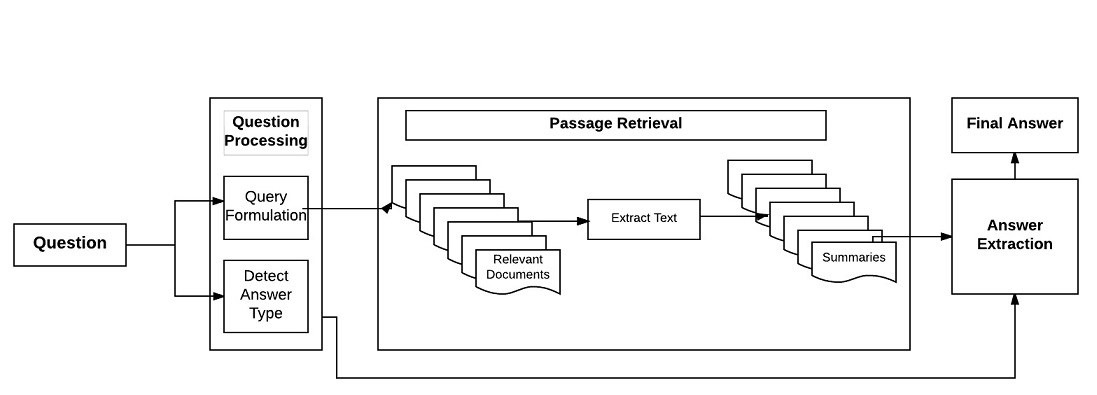
\includegraphics[scale=0.8]{images/IR_BasedQA.jpg}
\caption{IR Based Question Answer System.} 
\label{fig:IR_BasedQA}
\end{figure}

\begin{enumerate}	
\item Question Processing \\
This phase decides what type of question is being asked and subsequently which type of answer to 
extract. For question processing to work we need to perform the query formulation. Query formulation converts the posed question into a form which can be used in Information Retrieval. Once the form of the question is identified the exact answer type can be retrieved. 
	
\item Retrieving and Ranking Passage \\
Once we get a query format from Step 1, we can use this to search the answer in the documents.
We first rank the documents in which we find the probable answers, after this we rank the documents in which a match was not found, we do this by using user written rules or by using machine learning algorithms.

\break
\item Extracting Answers \\
The system extracts answers from passages using one of the two methods either by using answer type or by using N-grams tiling.
\end{enumerate}

\subsection{Knowledge based Question Answer System}
This paradigm relies on the mechanism to query a database. A semantic query is formed for the question which is asked. The query formed is used to retrieve result from the database. The system ideally functions like a semantic parser as it maps a text string to a logical format. The database can be a ususal relational database or the system may store triplets. The triplet has a predicate which defines the relation between the other 2 (two) parts. For example, DBPedia \cite{auer2007dbpedia}, Freebase \cite {bollacker2008freebase} are triplet stores derived from Wikipedia Infoboxes. One of the questions which can be posed to Knowledge based Question Answer system is to ask about one of the missing factors in the triplet. A Knowledge Based System can be implemented using the following approaches,

\begin{enumerate}

\item Rule Based Approach \\
This approach involves implementing hand written rules which will be used to extract the missing element from the triplet.
 
 \item Supervised Approach \\
In this approach, we have a training data consisting of mappings of questions to their logical forms. The model is trained using this data, so that going ahead it can identify which mapping to use in the future.
 
 \item Semi Supervised Approach \\
With the ruled based approach one needs to know the language for which the system is being implemented which cannot be the case always. For the supervised approach the most challenging aspect is having quality and correct training data, which always never happens. To overcome the drawbacks of these approaches we have a Semi supervised approach. One system known as REVERB extracts information from triplet stores and other sources like Wikipedia to create new relations while parallelly undergoing training to map between questions and the logical forms.

\end{enumerate}

\subsection{Hybrid Approach to Question Answering System}
The previous approaches were limited to using text or knowledge for the Question Answer System. In the hybrid approach we combine the steps in these to implement the system. One example of such a system is IBM Watson \cite {high2012era}. Figure 2 describes the different phases involved in the implementing a hybrid question answer system.

\begin{enumerate}

\item Question Processing \\
In this phase, the system parses the question, tags it for named entities and extracts possible relations and as in the IR based approach it detects the answer type and question type.

\begin{figure}[htb]
\centering
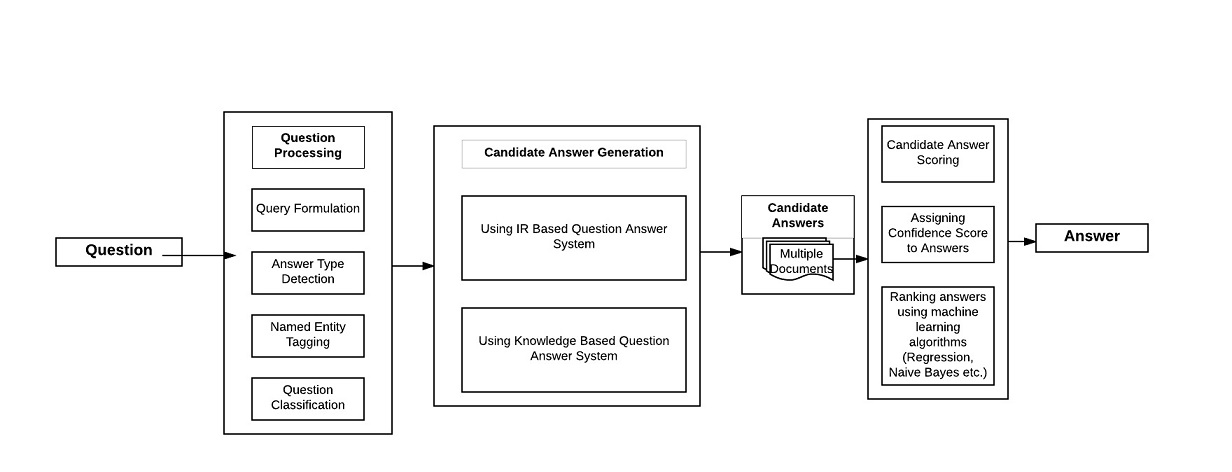
\includegraphics[scale=0.8]{images/Hybrid_QA.jpg}
\caption{Hybrid Question Answer System.} 
\label{fig:Hybrid_QA}
\end{figure}

\break
\item Candidate Answer Generation \\
Once we have the query phase from Step 1, we search external documents, texts and transcripts as well as a structured database to extract as many as possible candidate answers. The manner in which we search the query phrase will differ, for the searching the external sources the methods depends on the text we are searching. For the database, we can use queries similar to the ones we use with triplet stores like FreeBase, DBPedia etc.

\item Answer merging and scoring \\
This involves merging the extracted answers which are similar. For example, United States of America and U.S.A would be merged, this needs a dictionary with similar entities which can help detect this type of conflicts. At the end, there have a set of answers each with a feature vector. These are then subjected to a classifier and assigned a confidence value. This step runs iteratively helping output the best answer to the user.

 \end{enumerate}